\section{Architectural Overview}
\label{sec:architecture_overview}

Figure~\ref{fig:syssimx_architecture} shows the layered architecture of \syssimx{} and the delegation chain from user code through the framework to the external simulation backends.
The architecture is organized into four internal layers, adapter, core abstractions, system orchestration, and execution, each with a clearly defined responsibility.
Six design principles shaped this layering:
%
\begin{enumerate}[nosep]
  \item \textit{component-based decomposition,}
  \item \textit{tool-agnostic core with backend adapters,}
  \item \textit{separation of model and orchestration,}
  \item \textit{pluggable execution algorithms,}
  \item \textit{explicit and unit-aware interfaces, and}
  \item \textit{minimal required contract with optional capabilities.}
\end{enumerate}
%
Rather than discussing these principles in isolation, the following paragraphs introduce each layer of the architecture and explain the design decisions that motivated it.
The description proceeds from the bottom of Figure~\ref{fig:syssimx_architecture} upward, starting with the external tools and ending with the execution algorithms.

\begin{figure}[t]
  \centering
  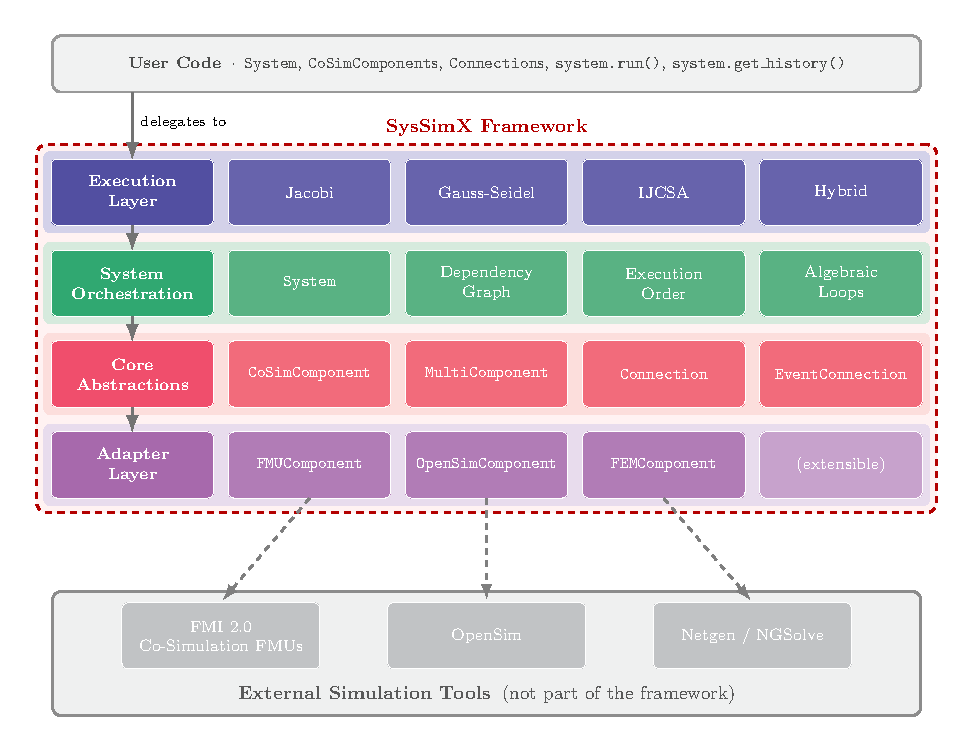
\includegraphics[width=\textwidth]{figures/4_architecture/syssimx_architecture.pdf}
  \caption{Layered architecture of the \syssimx{} framework.
  Solid arrows indicate the delegation direction between layers;
  dashed arrows indicate calls to external tool APIs across the
  framework boundary.}
  \label{fig:syssimx_architecture}
\end{figure}

\paragraph{External simulation tools.}
The simulation backends at the bottom of Figure~\ref{fig:syssimx_architecture} are not part of the framework.
They include FMI~2.0 Co-Simulation FMUs exported from equation-based modeling environments, OpenSim for musculoskeletal dynamics, and Netgen/NGSolve for finite element analysis.
Each tool provides its own solver, model representation, and programmatic Python interface.
The framework treats these tools as black-box backends and interacts with them exclusively through their respective APIs.

\paragraph{Adapter layer.}
The adapter layer wraps each tool-specific API in a class that implements the common  \texttt{CoSimComponent} interface.
\texttt{FMUComponent} maps FMI function calls to the component lifecycle.
\texttt{OpenSimComponent} wraps OpenSim in the same way.
For finite element models, \texttt{FEMComponent} marks the adapter slot but contributes minimal shared logic, since each FE model defines its own discretization, material law, and time integration scheme (Section~\ref{sec:impl_fem}).
As a result, every subsystem model, regardless of its origin, exposes the same interface for initialization, time stepping, input and output exchange, and state access.
This realizes the principle of a \emph{tool-agnostic core with backend adapters}.
All tool-specific code is confined to the adapter boundary, and the layers above can treat heterogeneous models uniformly.
The adapter layer is designed to be extensible. Additional backends can be integrated by providing a new adapter class without modifying the layers above.

\paragraph{Core abstractions.}
The core abstraction layer defines the modeling primitives of the framework.
The abstract base class \texttt{CoSimComponent} specifies the contract that every simulation component must satisfy. These are typed and unit-annotated input and output ports, a fixed lifecycle for initialization, stepping, and output evaluation, and optional hooks for direct-feedthrough declaration, event indicators, and state rollback.
This reflects two design principles.
First, \emph{component-based decomposition}, a system is represented as a set of interacting components that can be constructed, configured, and exchanged independently.
Second, \emph{minimal required contract with optional capabilities}, the component interface distinguishes between abstract methods that every component must implement and optional methods that enable participation in advanced framework features.
A simple component only needs to implement the core lifecycle methods.
Components that act as event sources must additionally implement state snapshot and rollback.
This keeps simple wrappers lightweight while allowing the framework to detect and exploit richer component capabilities where available.

Signal connections and event connections define the directed data flow and discrete event propagation between components.
\emph{Explicit and unit-aware interfaces} make coupling assumptions visible.
Each port carries a declared type and physical unit, and connections are validated for compatibility when they are added to the system.
The \texttt{MultiComponent} class extends this layer to the case where several interchangeable models represent the same physical subsystem, providing a single external interface while managing multiple internal realizations with consistent state synchronization.

\paragraph{System orchestration.}
The \texttt{System} class assembles components and connections into a complete co-simulation model.
It validates port compatibility, constructs the dependency graph, derives a topologically sorted execution order, identifies direct-feedthrough dependencies, and detects algebraic loops through strongly connected component analysis.
These structural properties are computed automatically during initialization and made available to the execution algorithms.
This layer embodies the \emph{separation of model and orchestration}.
Components are responsible for their own state integration and output evaluation, while the \texttt{System} class handles all system-level structural concerns.

\paragraph{Execution layer.}
The execution layer at the top of the framework contains the master algorithms that advance the coupled system in time.
An algorithm receives a \texttt{System} instance and steps all components from the current communication time~$t$ to~$t + \Delta t$, managing input propagation, output collection, and, where required, iterative resolution of algebraic loops or detection, localization, and handling of discrete events.
The same system model can be executed with different algorithms without modifying the component implementations or the system definition.
This realizes the principle of \emph{pluggable execution algorithms}.
The framework delegates all stepping logic to interchangeable algorithm objects, keeping numerical orchestration separate from model structure.

\paragraph{Supporting services.}
In addition to the main layers, the framework provides supporting services for unit handling, recording of port and component histories during simulation, and graph-based visualization of the system structure.

% The following sections describe each of the core abstractions in detail, beginning with the \texttt{CoSimComponent} interface.